\documentclass[14pt]{extbook}
\usepackage{multicol, enumerate, enumitem, hyperref, color, soul, setspace, parskip, fancyhdr} %General Packages
\usepackage{amssymb, amsthm, amsmath, latexsym, units, mathtools} %Math Packages
\everymath{\displaystyle} %All math in Display Style
% Packages with additional options
\usepackage[headsep=0.5cm,headheight=12pt, left=1 in,right= 1 in,top= 1 in,bottom= 1 in]{geometry}
\usepackage[usenames,dvipsnames]{xcolor}
\usepackage{dashrule}  % Package to use the command below to create lines between items
\newcommand{\litem}[1]{\item#1\hspace*{-1cm}\rule{\textwidth}{0.4pt}}
\pagestyle{fancy}
\lhead{Makeup Progress Quiz 2}
\chead{}
\rhead{Version A}
\lfoot{2790-1423}
\cfoot{}
\rfoot{Summer C 2021}
\begin{document}

\begin{enumerate}
\litem{
Determine the horizontal and/or oblique asymptotes in the rational function below.\[ f(x) = \frac{10x^{3} -59 x^{2} +61 x + 60}{-10x^{3} +3 x^{2} -27 x -36} \]\begin{enumerate}[label=\Alph*.]
\item \( \text{Horizontal Asymptote of } y = 0  \)
\item \( \text{Vertical Asymptote of } y = 1.500  \)
\item \( \text{None of the above} \)
\item \( \text{Horizontal Asymptote of } y = -1.000  \)
\item \( \text{Vertical Asymptote of } y = 4  \)

\end{enumerate} }
\litem{
Determine the vertical asymptotes and holes in the rational function below.\[ f(x) = \frac{8x^{3} -50 x^{2} +93 x -45}{8x^{2} -10 x -25} \]\begin{enumerate}[label=\Alph*.]
\item \( \text{Vertical Asymptote of } x = 1.0 \text{ and hole at } x = 2.5 \)
\item \( \text{Vertical Asymptote of } x = -1.25 \text{ and hole at } x = 2.5 \)
\item \( \text{Holes at } x = -1.25 \text{ and } x = 2.5 \text{ with no vertical asymptotes.} \)
\item \( \text{Vertical Asymptotes of } x = -1.25 \text{ and } x = 2.5 \text{ with no holes.} \)
\item \( \text{Vertical Asymptotes of } x = -1.25 \text{ and } x = 0.75 \text{ with a hole at } x = 2.5 \)

\end{enumerate} }
\litem{
Which of the following functions \textit{could} be the graph below?
\begin{center}
    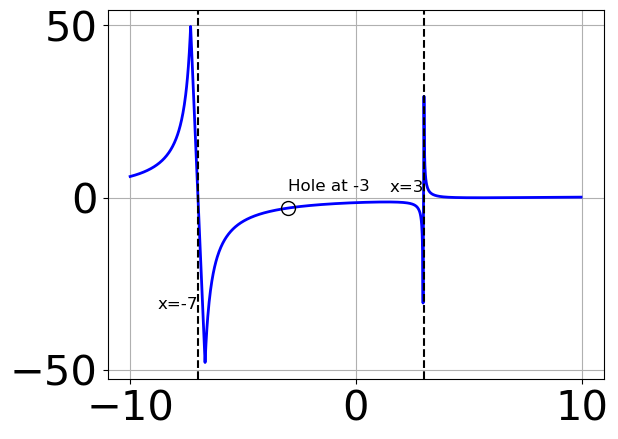
\includegraphics[width=0.5\textwidth]{../Figures/identifyGraphOfRationalFunctionCopyA.png}
\end{center}
\begin{enumerate}[label=\Alph*.]
\item \( f(x)=\frac{x^{3} +8.0 x^{2} -3.0 x -90.0}{x^{3} -7.0 x^{2} -9.0 x + 63.0} \)
\item \( f(x)=\frac{x^{3} -8.0 x^{2} -3.0 x + 90.0}{x^{3} +7.0 x^{2} -9.0 x -63.0} \)
\item \( f(x)=\frac{x^{3} +13.0 x^{2} +52.0 x + 60.0}{x^{3} -7.0 x^{2} -9.0 x + 63.0} \)
\item \( f(x)=\frac{x^{3} -10.0 x^{2} +19.0 x + 30.0}{x^{3} +7.0 x^{2} -9.0 x -63.0} \)
\item \( \text{None of the above are possible equations for the graph.} \)

\end{enumerate} }
\litem{
Determine the horizontal and/or oblique asymptotes in the rational function below.\[ f(x) = \frac{12x^{3} -65 x^{2} +74 x -24}{3x^{2} -11 x + 6} \]\begin{enumerate}[label=\Alph*.]
\item \( \text{Oblique Asymptote of } y = 4x -7. \)
\item \( \text{Horizontal Asymptote of } y = 4.0 \text{ and Oblique Asymptote of } y = 4x -7 \)
\item \( \text{Horizontal Asymptote of } y = 3.0 \text{ and Oblique Asymptote of } y = 4x -7 \)
\item \( \text{Horizontal Asymptote of } y = 4.0  \)
\item \( \text{Horizontal Asymptote at } y = 3.0 \)

\end{enumerate} }
\litem{
Which of the following functions \textit{could} be the graph below?
\begin{center}
    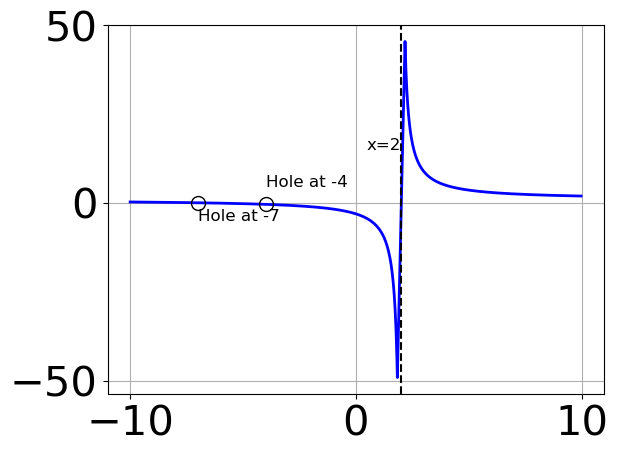
\includegraphics[width=0.5\textwidth]{../Figures/identifyGraphOfRationalFunctionA.png}
\end{center}
\begin{enumerate}[label=\Alph*.]
\item \( f(x)=\frac{x^{3} +14.0 x^{2} +63.0 x + 90.0}{x^{3} +9.0 x^{2} +6.0 x -56.0} \)
\item \( f(x)=\frac{x^{3} +17.0 x^{2} +94.0 x + 168.0}{x^{3} +9.0 x^{2} +6.0 x -56.0} \)
\item \( f(x)=\frac{x^{3} -17.0 x^{2} +94.0 x -168.0}{x^{3} -9.0 x^{2} +6.0 x + 56.0} \)
\item \( f(x)=\frac{x^{3} -7.0 x^{2} -24.0 x + 180.0}{x^{3} -9.0 x^{2} +6.0 x + 56.0} \)
\item \( \text{None of the above are possible equations for the graph.} \)

\end{enumerate} }
\litem{
Determine the vertical asymptotes and holes in the rational function below.\[ f(x) = \frac{8x^{3} -18 x^{2} -11 x + 30}{16x^{2} +32 x + 15} \]\begin{enumerate}[label=\Alph*.]
\item \( \text{Vertical Asymptotes of } x = -0.75 \text{ and } x = 1.5 \text{ with a hole at } x = -1.25 \)
\item \( \text{Vertical Asymptote of } x = -0.75 \text{ and hole at } x = -1.25 \)
\item \( \text{Vertical Asymptote of } x = 0.5 \text{ and hole at } x = -1.25 \)
\item \( \text{Vertical Asymptotes of } x = -0.75 \text{ and } x = -1.25 \text{ with no holes.} \)
\item \( \text{Holes at } x = -0.75 \text{ and } x = -1.25 \text{ with no vertical asymptotes.} \)

\end{enumerate} }
\litem{
Determine the horizontal and/or oblique asymptotes in the rational function below.\[ f(x) = \frac{9x^{3} -18 x^{2} -64 x -32}{3x^{2} +19 x + 20} \]\begin{enumerate}[label=\Alph*.]
\item \( \text{Horizontal Asymptote of } y = -5.0 \text{ and Oblique Asymptote of } y = 3x -25 \)
\item \( \text{Horizontal Asymptote of } y = 3.0 \text{ and Oblique Asymptote of } y = 3x -25 \)
\item \( \text{Horizontal Asymptote at } y = -5.0 \)
\item \( \text{Horizontal Asymptote of } y = 3.0  \)
\item \( \text{Oblique Asymptote of } y = 3x -25. \)

\end{enumerate} }
\litem{
Determine the horizontal and/or oblique asymptotes in the rational function below.\[ f(x) = \frac{15x^{3} +26 x^{2} -51 x + 18}{-15x^{3} +8 x^{2} +3 x + 18} \]\begin{enumerate}[label=\Alph*.]
\item \( \text{Vertical Asymptote of } y = -0.667  \)
\item \( \text{None of the above} \)
\item \( \text{Horizontal Asymptote of } y = 0  \)
\item \( \text{Vertical Asymptote of } y = -3  \)
\item \( \text{Horizontal Asymptote of } y = -1.000  \)

\end{enumerate} }
\litem{
Determine the vertical asymptotes and holes in the rational function below.\[ f(x) = \frac{9x^{3} -24 x^{2} +4 x + 16}{12x^{2} +23 x + 10} \]\begin{enumerate}[label=\Alph*.]
\item \( \text{Holes at } x = -1.25 \text{ and } x = -0.667 \text{ with no vertical asymptotes.} \)
\item \( \text{Vertical Asymptotes of } x = -1.25 \text{ and } x = -0.667 \text{ with no holes.} \)
\item \( \text{Vertical Asymptotes of } x = -1.25 \text{ and } x = 1.333 \text{ with a hole at } x = -0.667 \)
\item \( \text{Vertical Asymptote of } x = 0.75 \text{ and hole at } x = -0.667 \)
\item \( \text{Vertical Asymptote of } x = -1.25 \text{ and hole at } x = -0.667 \)

\end{enumerate} }
\litem{
Determine the vertical asymptotes and holes in the rational function below.\[ f(x) = \frac{9x^{3} -18 x^{2} -7 x + 20}{6x^{2} +7 x -20} \]\begin{enumerate}[label=\Alph*.]
\item \( \text{Vertical Asymptotes of } x = -2.5 \text{ and } x = 1.667 \text{ with a hole at } x = 1.333 \)
\item \( \text{Vertical Asymptote of } x = 1.5 \text{ and hole at } x = 1.333 \)
\item \( \text{Vertical Asymptotes of } x = -2.5 \text{ and } x = 1.333 \text{ with no holes.} \)
\item \( \text{Vertical Asymptote of } x = -2.5 \text{ and hole at } x = 1.333 \)
\item \( \text{Holes at } x = -2.5 \text{ and } x = 1.333 \text{ with no vertical asymptotes.} \)

\end{enumerate} }
\end{enumerate}

\end{document}